\section{Problem Statement}
\label{sec:problemStatement}

\begin{figure}[t]
\centering
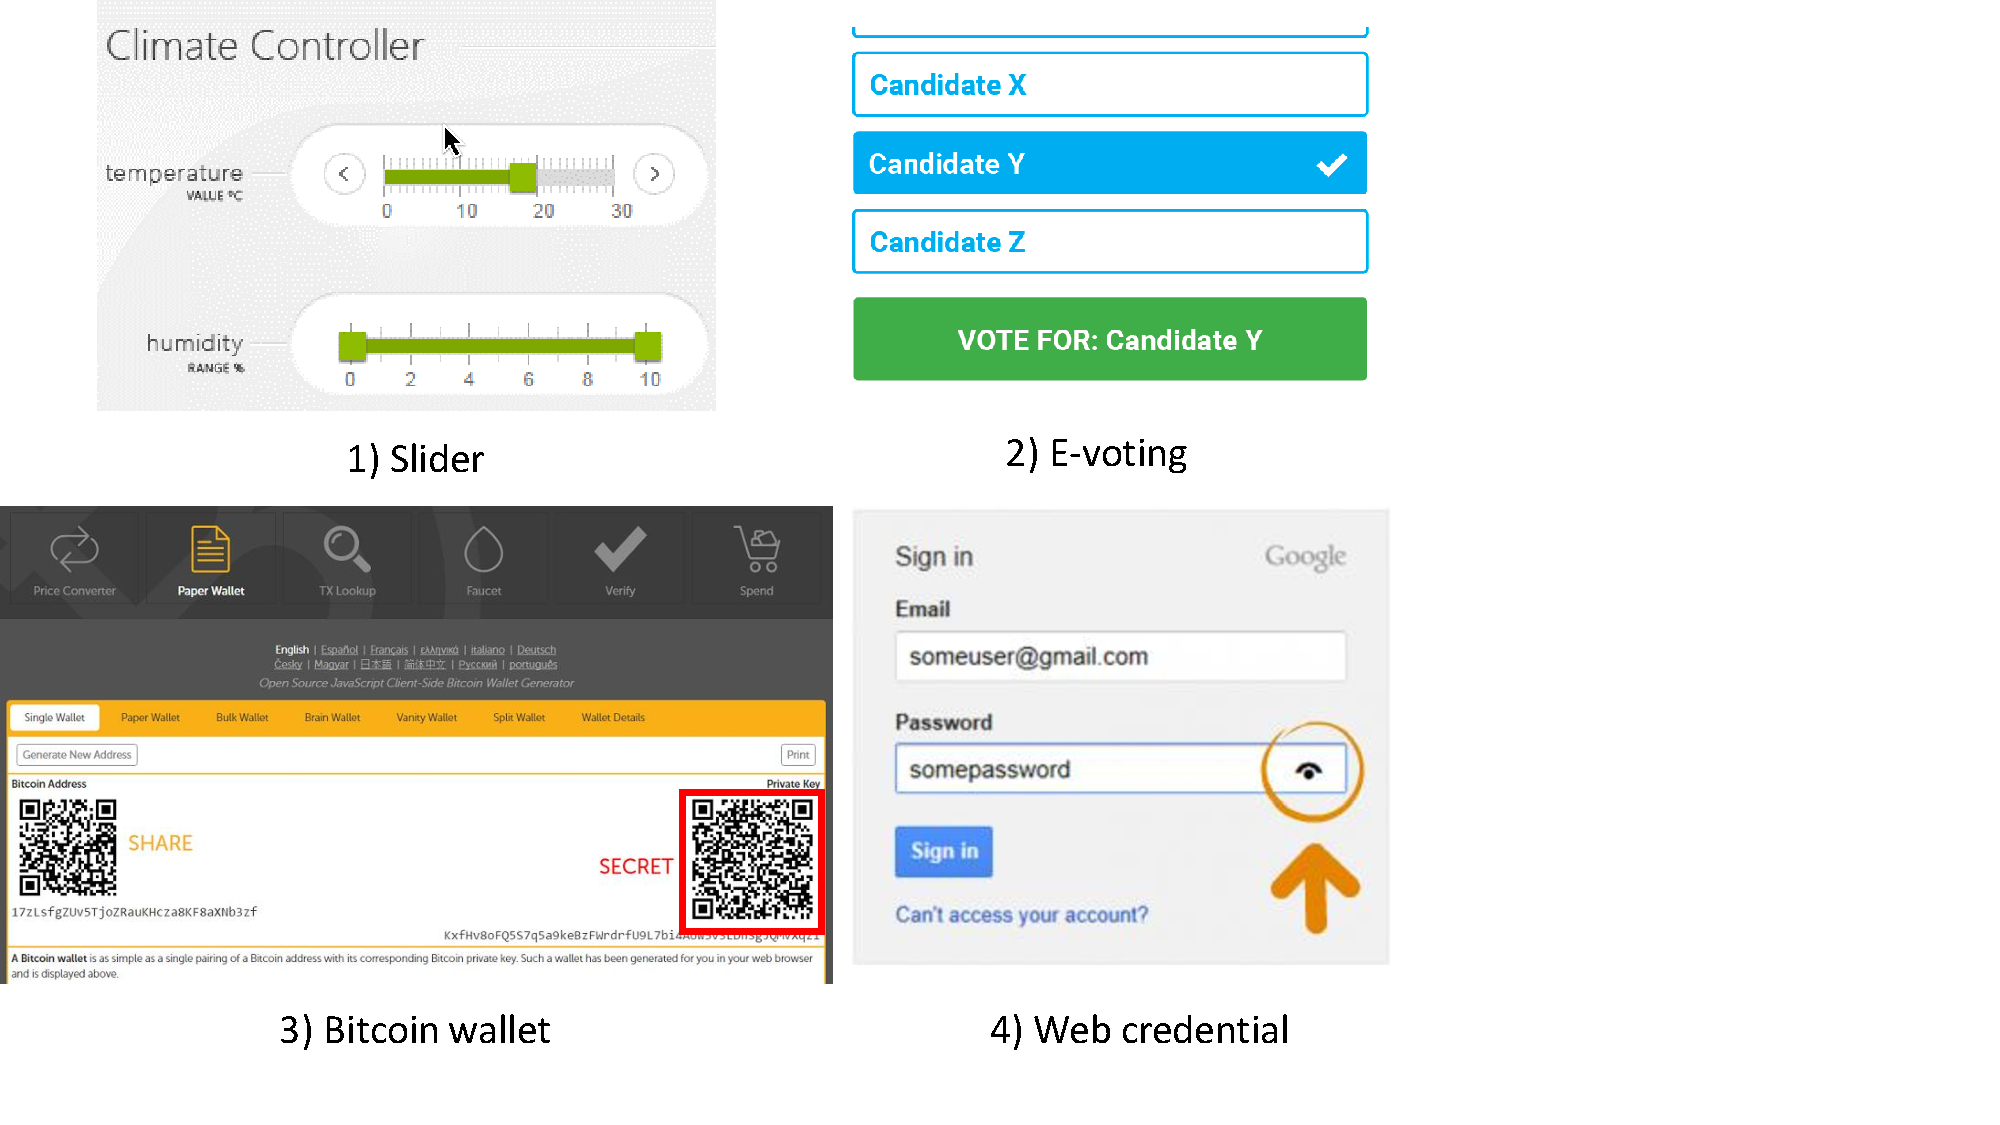
\includegraphics[trim={0 1cm 10cm 0}, clip, width=\linewidth]{motivation.pdf}
\caption{\textbf{Motivating examples.} 1) Pointer based UI elements that sets parameters to remote safety-critical device, 2) E-voting where the voting privacy and integrity is critical, 3) Financial transactions such as bitcoin wallet that shows sensitive information such as the user's private key and 4) web applications that provide an option for the user to reveal credentials.}
\label{fig:motivation}
\centering
\end{figure}


\subsection{Motivation and Problem Statement}

Input and output integrity and privacy is a crucial problem when one assumes the attacker model where the attacker compromises host systems that include the hardware, the operating systems, and all the installed applications. Such an attacker model allows it not only to steal the sensitive information from the user but also alter them. Furthermore, the user is completely unprotected, she  cannot verify that her inputs are transferred to the server securely, or even have the guarantee that she is communicating with the legitimate server.

The attacker can easily change system configurations (i.e., install root certificates), alter user's transaction, or manipulate the user by showing false information on the screen. Figure~\ref{fig:motivation} provides four such cases where the secrecy and the integrity of the input and output data are crucial. Effectively the primary motivation of this work is to build an efficient and effective \emph{trusted path} solution that provides highest from of security in terms of integrity and privacy.  
Based on these examples we list 6 security properties that we want to provide in our propose solution. We now discuss these security properties and corresponds them with the motivating example.

\begin{enumerate}
  \item \textbf{Input integrity.} In a case where the user provides input to a remote safety-critical system, input integrity is a crucial property that ensures that the command from the user reaches to the remote end-point without any modification by the malicious host system. Case 1 in Figure~\ref{fig:motivation} is a concrete example where input integrity is critical for the application to be work properly.
  \item \textbf{Input privacy.}  Input privacy is required if the malicious host wants to steal the sensitive information from the user. This involves the credentials for various web-service, financial information such as the credit card number, choice of the vote in the e-voting system. Cases 2,3,and 4 in Figure~\ref{fig:motivation} are the example where input privacy is needed.
  \item \textbf{Output integrity.} Output integrity is a critical component to ensure a secure display. This involves data coming from remote safety-critical devices, medical implants, financial data such as the bitcoin address, candidate list in the e-voting portal etc. Cases 1,2, and 3 in Figure~\ref{fig:motivation} are the potential scenarios where output integrity property is desirable.
  \item \textbf{Output privacy.} In many application scenarios, output privacy is required where the data sent from the remote end-point is privacy sensitive. Such includes the web credentials, candidate preference data in the e-voting, the private key of the bitcoin wallet etc. Example scenarios 2,3 and 4 in Figure~\ref{fig:motivation} require output privacy.
  \item \textbf{Activity privacy.} We define activity analogously to the user intention which is privacy sensitive in many application scenarios. One such concrete example is e-voting where voting privacy is of uttermost importance. Even if there is a system in place that provides input privacy, merely the fact that the user may hover her mouse over some candidates may reveal her candidate preference. Activity privacy is application specific and in most of the case, it dynamically preserves a part of the scene where the user activity is oblivious to the compromised host. 
\end{enumerate}


\iffalse
\myparagraph{Advantages}

\begin{enumerate}
  \item The \device does not need to know the formatting/template of the page. As the \device only looks to the current mouse position, the structure of the page is somewhat irrelevant (?).
\end{enumerate}
\fi


\subsection{Potential Solutions and their drawbacks}

Given the attacker's model, there exist several solutions that solve the problem of a trusted path to and from the IO devices in the presence of a compromised host. But all of these solutions targeted for different problem settings and models:

\myparagraph{Strawman solution: trusted OS.} Trusted OS could be seen as a straightforward solution as traditionally OS handles all the IO drives, computation, and network communications. Assuming a trusted OS significantly reduces the complexity of the solution but the security assumption suffers. Trusted OS introduces a large trusted code base and a multitude of vulnerabilities. 

\myparagraph{Trusted Execution Environment.} TEEs are another ways to implement a trusted path between the IO devices and the users. Several TEEs such as Intel SGX, ARM TrustZone, TPM, Intel TXT etc. can be used to achieve such functionality. Several research works such as Intel SGX and trusted hypervisor based SGXIO~\cite{weiser2017sgxio}, Intel SGX based ProximiTEE~\cite{dhar2018proximitee}, TPM and TXT based trusted path~\cite{filyanov2011uni} and ARM TrustZone based trusted path~\cite{filyanov2011uni,sun2015trustotp} are the example of trusted path construction based on TEEs. All of these solutions require specialized platforms with processors that support such infrastructure. In our proposed solution, we concentrate on the non-specialized hardware platform where compatible TEE technologies may not be available.
Moreover, TEE requires trust assumption on the processors and additional code bases. One such example is INtel SGX where the trust model includes the physical processor package, SGX SDK, quoting enclave, launch enclave and Intel attestation service. Our proposed solution avoids such extensive trust assumptions and assumes that the entire platform is in control of the attacker.

\myparagraph{Hypervisor, hardware-based solutions.} Trusted hypervisors and secure micro-kernels are also choices for contrasting Trusted path. Sel4~\cite{klein2009sel4} is a functional hypervisor that is formally verified and has a kernel size of only $8400$ lines of code. (\textcolor{red}{copied from SGXIO paper})Work done by Zhou et al.~\cite{zhou2012building} builds a generic trusted path on $x86$ systems in a pure hypervisor-based design. They show the first comprehensive approach to x86 systems, protecting a trusted path all the way from the application level down to the device level.  They consider PCI device misconfiguration, DMA attacks as well as interrupt spoofing attacks.  However, pure hypervisor-based designs come at a price.  They strictly separate the untrusted stack from the trusted one.  Hence, the hypervisor is in charge of managing all secure applications and all associated resources itself.  This includes secure process and memory management with scheduling, verified launch, and attestation.  Also, communication between both security domains might be non-trivial due to synchronization issues or potentially mismatching Application Binary Interfaces (ABI).

\myparagraph{Dedicated hardware based solution.} Previous research works such as IntegriKey~\cite{IntegriKey} uses a low-TCB embedded device to introduce a second factor for input integrity. Fidelius~\cite{Fidelius} uses raspberry pi's and Intel SGX to create a secure channel between the keyboard and the display device. By doing so Fidelius provides secure input and secure display for character-based input. We inspired from Fidelius to extend it even further to generic IO operations for a wider range of UI elements. Note that extending input devices, such as from a keyboard to a mouse is not a trivial task. Without proper analysis of each and every frame that the host system produces, it is not possible to track user intention. In our knowledge, our proposed solution is the first to provide such security properties including the activity privacy. Moreover, we want to achieve this in the absence of any TEE as the trust model of our scenario is significantly different. 


\subsection{Goals}

In the above, we discussed several solutions and research works that solve the problem of constructing a trusted path in different ways. What makes our solution different from them is the specific settings that it targets. we do not assume trust on the OS, specific drivers, TEEs, hypervisors, etc. As all of these techniques as mentioned earlier requires trust on a large code base. Instead, our proposed solution solves the problem of building an efficient, trusted path using an off-the-shelf microcontroller and single board computers that requires bare-minimum trust assumption. The most distinguishing factor is the type of IOs our proposed system targets to protect, namely mouse/touch inputs and sophisticated user interfaces. Existing research works primarily targets character-based input devices such as keyboards, and the methods cannot be trivially applied to mouse/touch-based inputs or complex UI elements. 

The goals are the following:

\begin{enumerate}
  \item \textbf{Easy deployment and integration.} Our proposed solution focuses on deploying it to existing system without any major changes. This also ensures minimal or no changes to the user interaction with the systems.
  \item \textbf{Security.} Our proposed solution provides IO and activity integrity and privacy to protect user provided data. This means that while deployed, the device always protects the integrity of user input and in specific application scenarios, it provides IO privacy and integrity.
\end{enumerate}


